
\chapter{绪\quad 论}
此处格式已按模板设定,作者只需选择段落区域,输入替换之。模版中所有说明性文字用于注释格式与内容的要求,撰写论文时请删除。模版中,图表、公式、参考文献等都已给出范例,撰写论文时请删除。

硕士学位论文一般要求不少于3万字;博士学位论文一般不少于5万字。除外语类相关专业外,学位论文正文应采用中文简体字撰写。正文的内容一般包括:国内外研究现状、理论分析、计算方法、实验装置和测试方法、实验结果分析与讨论、研究成果、结论及意义。

章节与标号:一般分为章标题(一级标题)、不编号章标题(同属于一级标题)、二级标题和三级标题。各章节编号建议采用Word的“多级别列表”方式自动形成编号,标题编号与标题内容之间空1个半角空格。各级章节标题格式要求细节参见《天津大学机械工程学院关于研究生学位论文统一格式的规定》。
本模版已包含符合上述章节设置的“多级别列表”,只需在相应位置替换标题文字即可。如需增加章节,建议先使用格式刷,再调整编号。

\section{正文格式规定}
正文文字两端对齐,首行缩进2字符,行间距为1.25行,段前0.2行,段后0行,孤行控制,自动调整中文与英文和数字的间距。正文中文字体采用宋体,字号为小四,英文和数字采用Times New Roman,字号为小四(12磅)。非英文字符,采用插入符号的方式。

中文部分应按照国家有关规定使用中文标点符号,英文部分使用西文标点符号并在其后加半角空格。当括号中仅包含英文和数字时使用西文括号并在其与中文之间增加半角空格。

正文中的变量和参数严格执行GB3100-3102:93有关量和单位的规定(具体要求请参阅《常用量和单位》. 计量出版社, 1996),一般应使用国际单位制。单位名称的书写,可采用国际通用符号,也可以用中文名称,但全文应统一,不可两种混用。正文中变量和参数等符号,字体字号基本与正文格式一致。非英文字符采用插入符号的方式,尽量避免使用行内公式,若必须使用行内公式,该段落行距可设为“最小值20磅”。数字与非中文符号、单位之间增加半角空格。

正文中图、表与正文之间要有1个空行的间距;文中的图、表、附注、公式一律采用阿拉伯数字分章编号, 章节号和编号之间用“-”连接。如:图2-5,表3-2,公式(5-1)等。若图或表中有附注,采用英文小写字母顺序编号;子图采用英文字母编号。正文中的行间公式、插图、表格的具体规定如下。

所有参考文献需要在正文后依照出现的先后顺序列出,并在正文中全部引用。引用方式例如:文献[1]的实验工作表明,Kasper等所建立的理论模型的正确性[2].

本模版包含已设置好的正文文字格式,只需在相应位置填写论文内容即可。

\subsection{行间公式}
\begin{enumerate}
    \item[a.] 	公式要标准、通用,公式中变量和参数需给出解释。
    \item[b.] 	公式使用公式编辑器编辑,公式中字号为12磅。
    \item[c.] 	公式编号用西文括号括起右对齐,编号与公式间不加虚线。
    \item[d.] 	一般情况下,公式在行中无缩放显示,公式居中,其余与正文同。
\end{enumerate}

依照以上标准的行间公示范例如下。
\begin{equation}
    \begin{aligned}
        \begin{split}
            \sigma_{ij} &= C_{ijkl}\varepsilon_{kl} \\
            \varepsilon_{ij} &= S_{ijkl}\sigma_{kl}, i, j, k, l = 1-3
        \end{split}
    \end{aligned}
\end{equation}
其中,$\sigma_{ij}$为应力分量;$\varepsilon_{ij}$为应变分量;$C_{ijkl}$为弹性系数张量分量,且$C_{ijkl} = C_{jikl} = C_{ijlk} = C_{klij}$;同理$S_{ijkl}$为柔顺系数张量分量, 且满足$S_{ijkl} = S_{jikl} = S_{ijlk} = S_{klij}$。因为$C$与$S$为互逆张量,因此其分量之间满足以下关系:$S_{ijkl}C_{klpq} = \frac{1}{2} (\delta_{ip}\delta_{jq}+\delta{iq}\delta_{jp}),i, j, k, l, p, q = 1-3$。
% \begin{equation}
%     \begin{split}
%         \label{equation:empirical}
%         V(w) &= \sum_{i=1}^{N}l(y_i,H(x_i))\\
%         &=\sum_{i=1}^{N}\max(\xi,|y_i-H(x_i)|-\xi)
%     \end{split}
% \end{equation}

% \begin{subequations}
%     \label{eq:angle_horizontal}
%     \begin{equation}
%         \theta_{{\rm A}i} = \theta_{{\rm B}i} = D_x \cdot \cos\frac{\pi}{4},
%     \end{equation}
%     \begin{equation}
%         \theta_{{\rm C}i} = D_x \cdot \sin\frac{\pi}{4}.
%     \end{equation}
% \end{subequations}
\subsection{图}
\begin{enumerate}
    \item[a.] 图要精选、简明,切忌与表及文字表述重复。
    \item[b.] 图序及图名(包括中文名和英文名,中文在上,英文在下)居中置于图的下方并于图在同一页,无缩进,字号为五号,其余与正文同。
    \item[c.] 图中的文字、符号以及单位等注释,应同正文文字对应的表述形式一致。若没有对应的定义和表述,则首选中文。
    \item[d.] 图中字体中文可采用宋体、黑体,英文和数字采用Times New Roman或Arial字体。图中文字以其在Word文档中显示的尺寸\footnote{由于Word中插图(包括采用Word的插图工具绘制的和采用第三方软件绘制并导入到word中的图片、曲线图等)的尺寸可随意缩放,以及Word与其他软件在字号定义、显示比例等方面的不完全兼容等原因,论文中插图的字号大小、线宽等以其插入后在文档中显示的实际尺寸为准。},高度不小于8磅(相当于六号字)、不大于10.5磅(相当于五号)。
    \item[e.] 图中曲线、坐标、指示性箭头等各种线条,不小于0.25磅。
    \item[f.] 图中出现多种颜色的曲线、云图时,需做到黑白打印也能够正确区分。
    \item[g.] 插入图片分辨率不低于72 dpi。
\end{enumerate}

依照以上标准的插图范例如下。
%需要调用宏包sepackage{graphicx}
\begin{figure}[H]
    \centering
    \setlength{\abovecaptionskip}{5pt}
    \setlength{\belowcaptionskip}{2pt}
    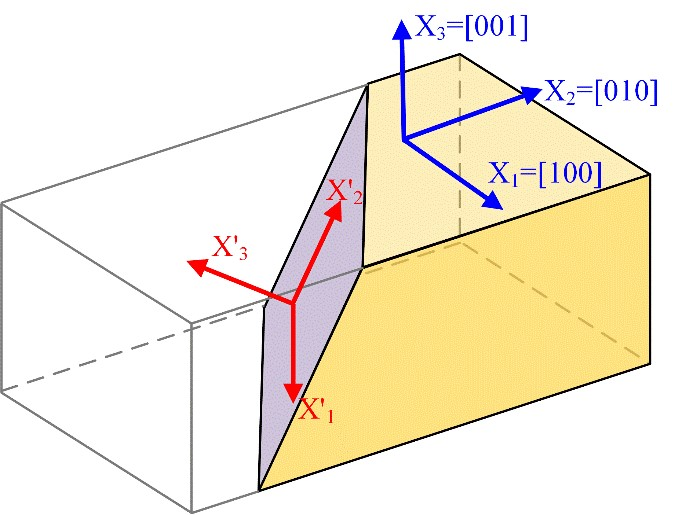
\includegraphics[scale=1]{figure1-1.jpg}
    %可选参数width=0.5inewidth
    \caption{晶体坐标系和样品坐标系示意图}
    \label{fig:figure1-1}
    \zihao{5}
    Figure\ \thefigure \ Illustration of crystal coordinate system and sample coordinate system
\end{figure}

%需要调用宏包sepackage{graphicx}
\begin{figure}[H]
    \centering
    \setlength{\abovecaptionskip}{5pt}
    \setlength{\belowcaptionskip}{2pt}
    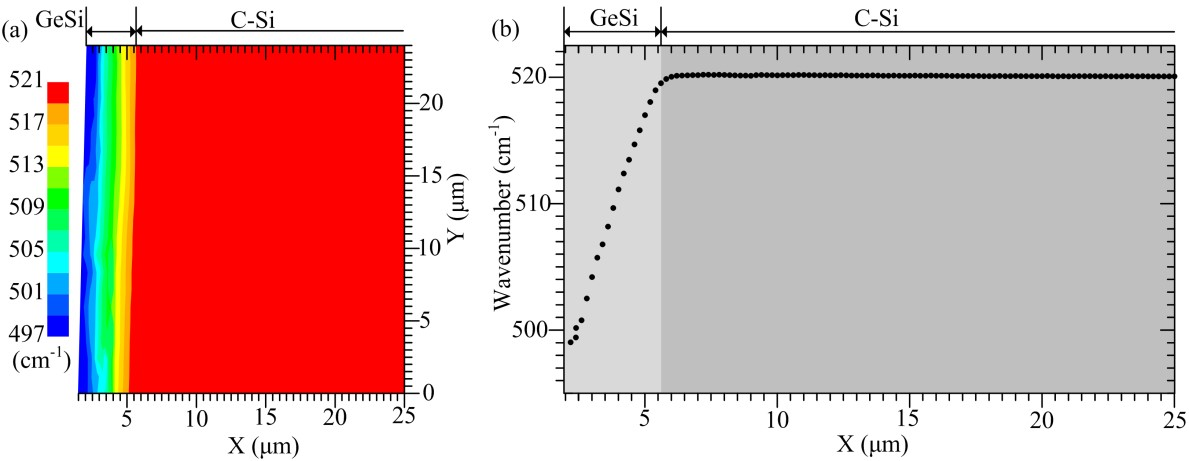
\includegraphics[scale=1]{figure1-2.jpg}
    %可选参数width=0.5inewidth
    \caption{应变硅横截面样品的拉曼类硅峰峰位 (a) 云图;(b) 沿深度方向分布曲线
    }
    \label{fig:figure1-2}
    \zihao{5}
    Figure\ \thefigure \ Wavenumber (a) image and (b) distribution along the depth direction on the cross-section sample
\end{figure}

%需要调用宏包sepackage{graphicx}
\begin{figure}[H]
    \centering
    \setlength{\abovecaptionskip}{5pt}
    \setlength{\belowcaptionskip}{2pt}
    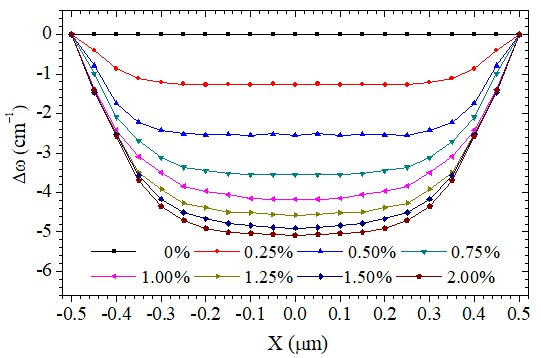
\includegraphics[scale=0.6]{figure1-3.jpg}
    %可选参数width=0.5inewidth
    \caption{不同基底应变状态下石墨烯样品沿长度方向波数分布}
    \label{fig:figure1-3}
    \zihao{5}
    Figure\ \thefigure \ Wavenumber distribution of graphene sample along length direction under different substrate strain
\end{figure}

\subsection{表}
\begin{enumerate}
    \item[a.] 表的编排采用国际通行的三线表,居中,无缩进。
    \item[b.] 表序及表名置于表的上方,居中无缩进,字号为五号,其余与正文同。
    \item[c.] 表名包括中文名和英文名,中文在上,英文在下。
    \item[d.] 表中文字居中无缩进,1.25行距,段前后间距为0,字号(包括文字、公式、变量、符号等)为五号,其余与正文同。
    \item[e.] 表中参数应标明量和单位的符号。
    \item[f.] 如需转页接排,在随后页上应重复表的编号和表题,并在表题后注明“(续)”,续表均应重复表头。
\end{enumerate}

依照以上标准的三线表范例如下。
%需要调用宏包\usepackage{booktabs}
\begin{table}[H]%需要调用宏包\usepackage{float}
    \renewcommand{\arraystretch}{1.5}%更改行距倍数
    \setlength{\abovecaptionskip}{2pt}
    \setlength{\belowcaptionskip}{5pt}
    \caption{tableCaption}
    \label{table:tableCaption}
    \centering
    \zihao{5}
    Table\ \thetable \ tableCaptionEn \vspace{2pt}\\%注意删除空格
    \begin{tabular}{ccc}
        \toprule
        实验方法     & 主要测量对象       & 空间分辨率          \\%注意删除空格
        \midrule
        原子力显微镜 & 表面力             & 0.1 nm\cite{dugang} \\%注意删除空格
        透射电镜     & 晶格结构、位错     & 0.1 nm              \\
        X射线衍射    & 应变               & 1 \si{\micro}m      \\
        同步辐射     & 内部三维结构与变形 & 约100 nm            \\
        显微拉曼     & 应变               & 250 nm              \\
        \bottomrule
    \end{tabular}
\end{table}


